\chapter{Controlling des Qualitätssicherungsprozesses}

    %  Dieses Kapitel zeigt Möglichkeiten den Prozess  der Qualitätssicherung zu bewerten und somit sicherzustellen, dass die resultierende Software eine hohe Qualität innehat. Dies kann anhand einer Umfrage unter fachkundigen Kollegen oder anhand von Kennzahlen geschehen .

    %  (Wird der Prozess bewertet oder die Ergebnisse des Prozesses? Eventuell beide Kontrollmethoden ausführen.

    Im vorherigen Kapitel wurden agile Prozesse beleuchtet und Methoden der Qualitätssicherung aufgeführt, die sicherstellen, dass auch in einem agilen Rahmen die betrachteten Charakteristiken von Softwarequalität erreicht werden. Der um die zuvor eingeführten agilen Methoden erweiterte Scrum-Prozess wird nun unter die Kontrolle eines Qualitätssicherungssystems wie Six Sigma gestellt, um die korrekte, vollständige und effiziente Umsetzung zu gewährleisten.

    Wie in \autoref{subsec:sixsigma} erwähnt folgt das Verfahren einem erweiterten Deming-Kreis, der die 5 Phasen Define, Measure, Analyse, Improve, Check vorsieht. Das folgenden Unterkapitel werden ebenfalls nach diesem Kreis aufgebaut sein und zeigen, wie die einzelnen Phasen auf Scrum angewandt werden können.

    \section{Define}

        Six Sigma schreib vor, dass zu Beginn des Prozesses die Anforderungen des Kunden aufzunehmen um daraus Aufgaben zu entwickeln deren Erfüllung messbar ist.
        \autoref{abb:define} zeigt die Schritte der Define Phase. Sie veranschaulicht, dass die Meinung des Kunden genauer spezifiziert wird, bis das ideale Ergebnis des Prozesses feststeht. Die Basis diese Prozesses bilden Kundenäußerungen, die das Produkt betreffen, aber auch Werte und Einstellungen des Kunden, die dem Zielprodukt nicht direkt zuzuordnen sind.

        Hieraus werden die Bedürfnisse des Kunden abgeleitet und in messbare Kriterien für die Software übersetzt. Dies soll sicherstellen, dass Erfüllung der Kundenbedürfnisse am Ende des Prozesses überprüft werden kann. Die \emph{Project Ys}, die oben in der Abbildung zu sehen sind geben die Kriterien an, an denen der Projekterfolg letztendlich gemessen wird.\footnote{Vgl. Knöfel, 2009, S.48.}

        \begin{figure}[!htbp]%[H]
            \begin{center}
                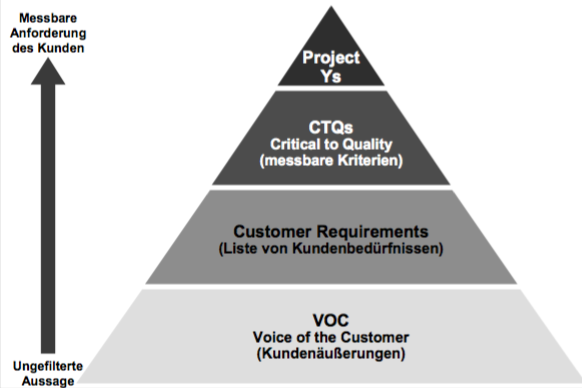
\includegraphics[width=11cm]{Abbildungen/define}
                \caption{Schritte der Definition\protect\footnotemark}
                \label{abb:define}
            \end{center}
        \end{figure}

        \footnotetext{Knöfel, 2009, S.44.}

        Im Scrum Verfahren werden im Gespräch mit dem Kunden Anforderungen herausgearbeitet und im Product Backlog festgehalten. Die Kundenäußerungen werden somit in eine Liste von Kundenbedürfnissen übertragen. Das Fundament der Define Phase wird somit durch die Rahmenbedingungen von Scrum gelegt und nun müssen diese Kundenbedürfnisse messbar gemacht werden.

        Die \emph{Definition of Done}, die anzeigen sollte, ob ein Kriterium messbar umgesetzt ist verfehlt hier allerdings die Intention des Six Sigma Verfahrens. Die Definition of Done bezieht sich darauf, dass bei einem Softwareprodukt nicht nur die Entwicklung, sondern auch Tests, Dokumentation und weiteres abgeschlossen ist, während ein messbares Kriterium Wünsche des Kunden, wie zum Beispiel \enquote{Eine schnelle Software!} in messbare Kriterien, wie \enquote{Eine Antwort auf meine Eingabe in weniger als 7 Sekunden!} beinhaltet. Neben der Funktion, die die Software erfüllt und die im Backlog festgehalten werden muss sollte das Entwicklungsteam daher auch implizite Anforderungen des Kunden festhalten und notieren.

        Die messbaren Kriterien ergänzen somit die Definition of Done. Der letzte Schritt der Definitionsphase sieht vor, dass die messbaren Kriterien priorisiert werden, um das Entwicklungsteam nicht zu überfordern. Für jede Anforderung im Product Backlog könnte daher ein eigener Backlog erstellt werden, der die messbaren Kriterien zur Erfüllung dieser Verantwortung priorisiert verwaltet.

        Somit besteht neben dem im Scrum üblichen Backlog ein weiterer Backlog je Anforderung, dass priorisierte, messbare Anforderungen liefert, wann das Hauptbacklogitem als erfüllt so betrachten ist.

        \begin{table}
        \label{tbl:checkDefine}
        \begin{tabularx}{\textwidth}{|p{3.5cm}|X|c|}
          \hline
          Schritt & Umsetzung & Erledigt \\
          \hline
          Kundenäußerungen aufnehmen & Wünsche des Kunden werden vom Product Owner im Product Backlog festgehalten. & $\Box$ \\
          &&\\
          Kundenbedürfnisse auflisten & Das Scrum-Team formuliert die Äußerungen in To-Dos und ergänzt mit diesen den Product Backlog. & $\Box$ \\
          &&\\
          Festlegen der Definition of Done & Das Scrum-Team legt intern fest, welche Schritte abgeschlossen sein müssen, damit die Entwicklung einer Iteration als fertig angesehen wird. & $\Box$ \\
          &&\\
          Kundenbedürfnisse in messbare Kriterien übersetzen & Das Scrum-Team legt in Zusammenarbeit mit dem Kunden SMARTe\footnotemark Ziele fest. & $\Box$ \\
          &&\\
          Kriterien zur Erfüllung von Bedürfnissen priorisieren & Für jeden Product Backlog Eintrag wird ein priorisierter Kriterienbacklog angelegt & $\Box$ \\
          &&\\
          Festlegen der wichtigsten Projektziele & Der Product Backlog wird nach der Wichtigkeit für den Kunden priorisiert & $\Box$ \\
          \hline
        \end{tabularx}
        \caption{Checkliste zum Abschluss der Define Phase}
        \end{table}

        \footnotetext{Siehe Glossar.}

        In \autoref{tbl:checkDefine} werden die Schritte aufgelistet, die im Rahmen der Define Phase abgelaufen sein sollten, zusammen mit einer möglichen Umsetzung in Scrum.

    \section{Measure}
    \label{sec:measure}

% Was genau wollen wir messen?
% Wie ist das Ziel am besten zu messen und welche Arten von Daten haben wir?
% Wie gut oder schlecht läuft der aktuelle Prozess?
% Wie groß ist dsa zu beseitigende Problem wirklich?

        Nachdem im Rahmen der Design-Phase Ziele festgelegt wurden, die messbar sind, werden die zu erreichenden Ziele zu Beginn der Measure Phase weiter spezifiziert. Zusätzlich zum Produkt Backlog wurde zu jedem Bedürfnis des Kunden ein priorisierter Satz an Anforderungen im Anforderungsbacklog abgelegt. Aus diesem Anforderungsbacklog heraus werden nun in Absprache mit dem Kunden die Ziele gegriffen, die verfolgt werden sollen.\footnote{Knöfel, 2009, S. 72.}

        \begin{figure}[!htbp]%[H]
            \begin{center}
                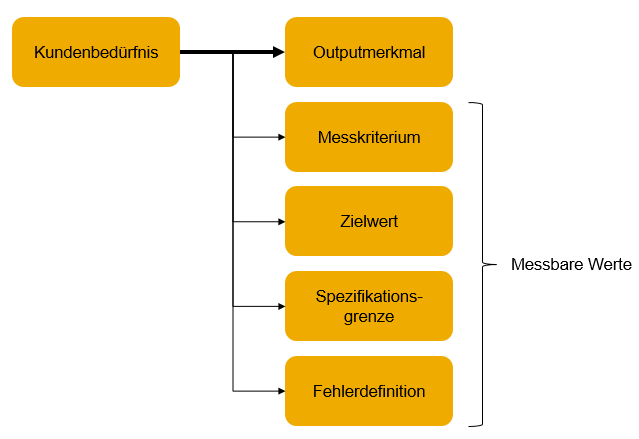
\includegraphics[width=11cm]{Abbildungen/ctq}
                \caption{Critical-To-Quality-Tree\protect\footnotemark}
                \label{abb:ctq}
            \end{center}
        \end{figure}

        \footnotetext{Eigene Abbildung in Anlehnung an Knöfel, 2009, S.73.}

        Jedes gewählte Element des Anforderungsbacklogs durchläuft nun den so genannten \emph{Critical-To-Quality-Tree}. Dieser ist in \autoref{abb:ctq} dargestellt. Die einzelnen Bestandteile des Baums werden an einem Beispiel für Verlässlichkeit der Softwarelösung dargestellt. Das Kundenbedürfnis \enquote{Das System soll eine sehr hohe Verfügbarkeit haben} würde durch folgende Punkte repräsentiert:

        Das Outputmerkmal ist der gemessene Wert, der in einem bestimmten Rahmen liegen soll. Für die Verfügbarkeit wäre dieser, die durchschnittliche Zeit pro Jahr, in der das System nicht erreichbar ist.

        Das Outputmesskriterium gibt an, wie das Outputmerkmal bestimmt wird. Im betrachteten Fall wäre dies das arithmetische Mittel der Zeit zwischen den Auftritten aller Systemausfälle bis zur Behebung eben dieser pro Jahr.

        Der Zielwert legt in Kombination mit der Spezifikationsgrenze die tolerierten Ergebnisse fest. Das Ergebnis sollte sich möglichst nahe des Zielwerts befinden, darf aber innerhalb der Grenzen von diesem abweichen, ohne, dass das Bedürfnis als nicht erfüllt gilt. Als Zielwert können maximal 12h pro Jahr festgelegt werden, an denen das System nicht erreichbar ist mit einer Toleranz von 12h pro Jahr. Für den Fehlerfall hieße dies, dass ab 24h Downtime pro Jahr das Kundenbedürfnis nicht erfüllt ist.

        Um zurück auf die Six Sigma Spezifikation aus \autoref{subsec:sixsigma} zu kommen bedeutet es für das oben gezeigte Beispiel, dass die Wahrscheinlichkeit, dass das System länger als 24h nicht erreichbar ist bei unter 0,0001\% liegt.

        Sollten zu einem Kundenbedürfnis mehrere Outputmerkmale bestehen werden alle in die Fehlerbetrachtung einbezogen.

        Im Anschluss ist es wichtig ein angemessenes Messverfahren zu finden und die Daten zu erheben. Auf die Auswahl des Messverfahrens wird im Rahmen dieser Arbeit nicht eingegangen, da dies den geplanten Umfang eben dieser überschreiten würde.
        Die Daten sollten nach der Messung digitalisiert oder digital erhoben werden, um eine effiziente Verarbeitung eben dieser zu ermöglichen.

        \begin{table}
        \label{tbl:checkDefine}
        \begin{tabularx}{\textwidth}{|p{3.5cm}|X|c|}
          \hline
          Schritt & Umsetzung & Erledigt \\
          \hline
          Ziele der Messung festlegen & Für jedes Element des Anforderungsbacklogs werden die Merkmale des Critical-To-Quality-Trees festgelegt. & $\Box$ \\
          &&\\
          Auswahl des Messverfahrens & Sicherstellen, dass reproduzierbare Messergebnisse mit geringer Varianz produziert werden & $\Box$ \\
          &&\\
          Messen der Merkmale & Die Merkmale werden gemessen und digitalisiert & $\Box$ \\
          \hline
        \end{tabularx}
        \caption{Checkliste zum Abschluss der Measure Phase}
        \end{table}

    \section{Analyze}
    
%        In der Analyse-Phase werden die relevanten Einflussfaktoren auf die Qualität des Endergebnisses herausgearbeitet.
%        Die Ursache von Fehlern, die im Produktionsprozess auftreten sollen gefunden werden.
        
        In der Analyse-Phase des Six Sigma Verfahren wird wert darauf gelegt die Ursachen für Fehler bei der Entwicklung festzustellen. Dies können bei der Entwicklung von Software unklare Anforderungen und Ziele sein, die eine nicht zu den Kundenbedürfnissen passende Software liefern oder Performancefehler, die durch Hard- oder Softwareoptimierungen zu erreichen wären.
        
        Um Fehler im Softwareentstehungsprozess zu entdecken müssen die Daten aus der Measure-Phase analysiert werden und die Ursachen für Fehler offen gelegt werden. Zu diesem Zweck wird das Beispiel aus dem \autoref{sec:measure} aufgegriffen.
        Zuletzt werden Verbesserungsmöglichkeiten herausgearbeitet.\footnote{Vgl. Knöfel, 2009, S.126.}

    \section{Improve}

    \section{Control} 